\documentclass[12pt,a4paper]{article}
\usepackage{graphicx}
\usepackage[dutch]{babel}
\usepackage[utf8]{inputenc}
\usepackage[margin=0.5in]{geometry}
\usepackage{amsmath}
\usepackage{amsfonts}
\usepackage{amssymb}
\usepackage{float}
\usepackage{hyperref}




\begin{document}
\graphicspath{{./images/}}
\DeclareGraphicsExtensions{.JPG}
\title{Stage verslag GNUDok}
\author{Silvio Bos}
\date{\today}
\maketitle
\section{Inleiding}
Ik loop stage bij het GNUDok, de ICT afdeling van het Juttersdok.
Hier bij GNUDok houden ze zich bezig met onderhoud, reparatie, systeembeheer en webdesign en levert computers en andere 
hardwarecomponenten voor de kringloopbedrijven van het juttersdok. 
Het is een erkend Leerbedrijf voor ICT op verschillende niveaus.
Ik heb bij het callcenter afspraken gemaakt, producten getest en computers klaargemaakt voor de verkoop.
Ik werk hier nu ongeveer 4-5 weken en ik vindt het een leuke stageplek omdat ik hier veel over ICT leer wat ik goed kan gebruiken in me opleiding.

\begin{figure}[H]
\centering
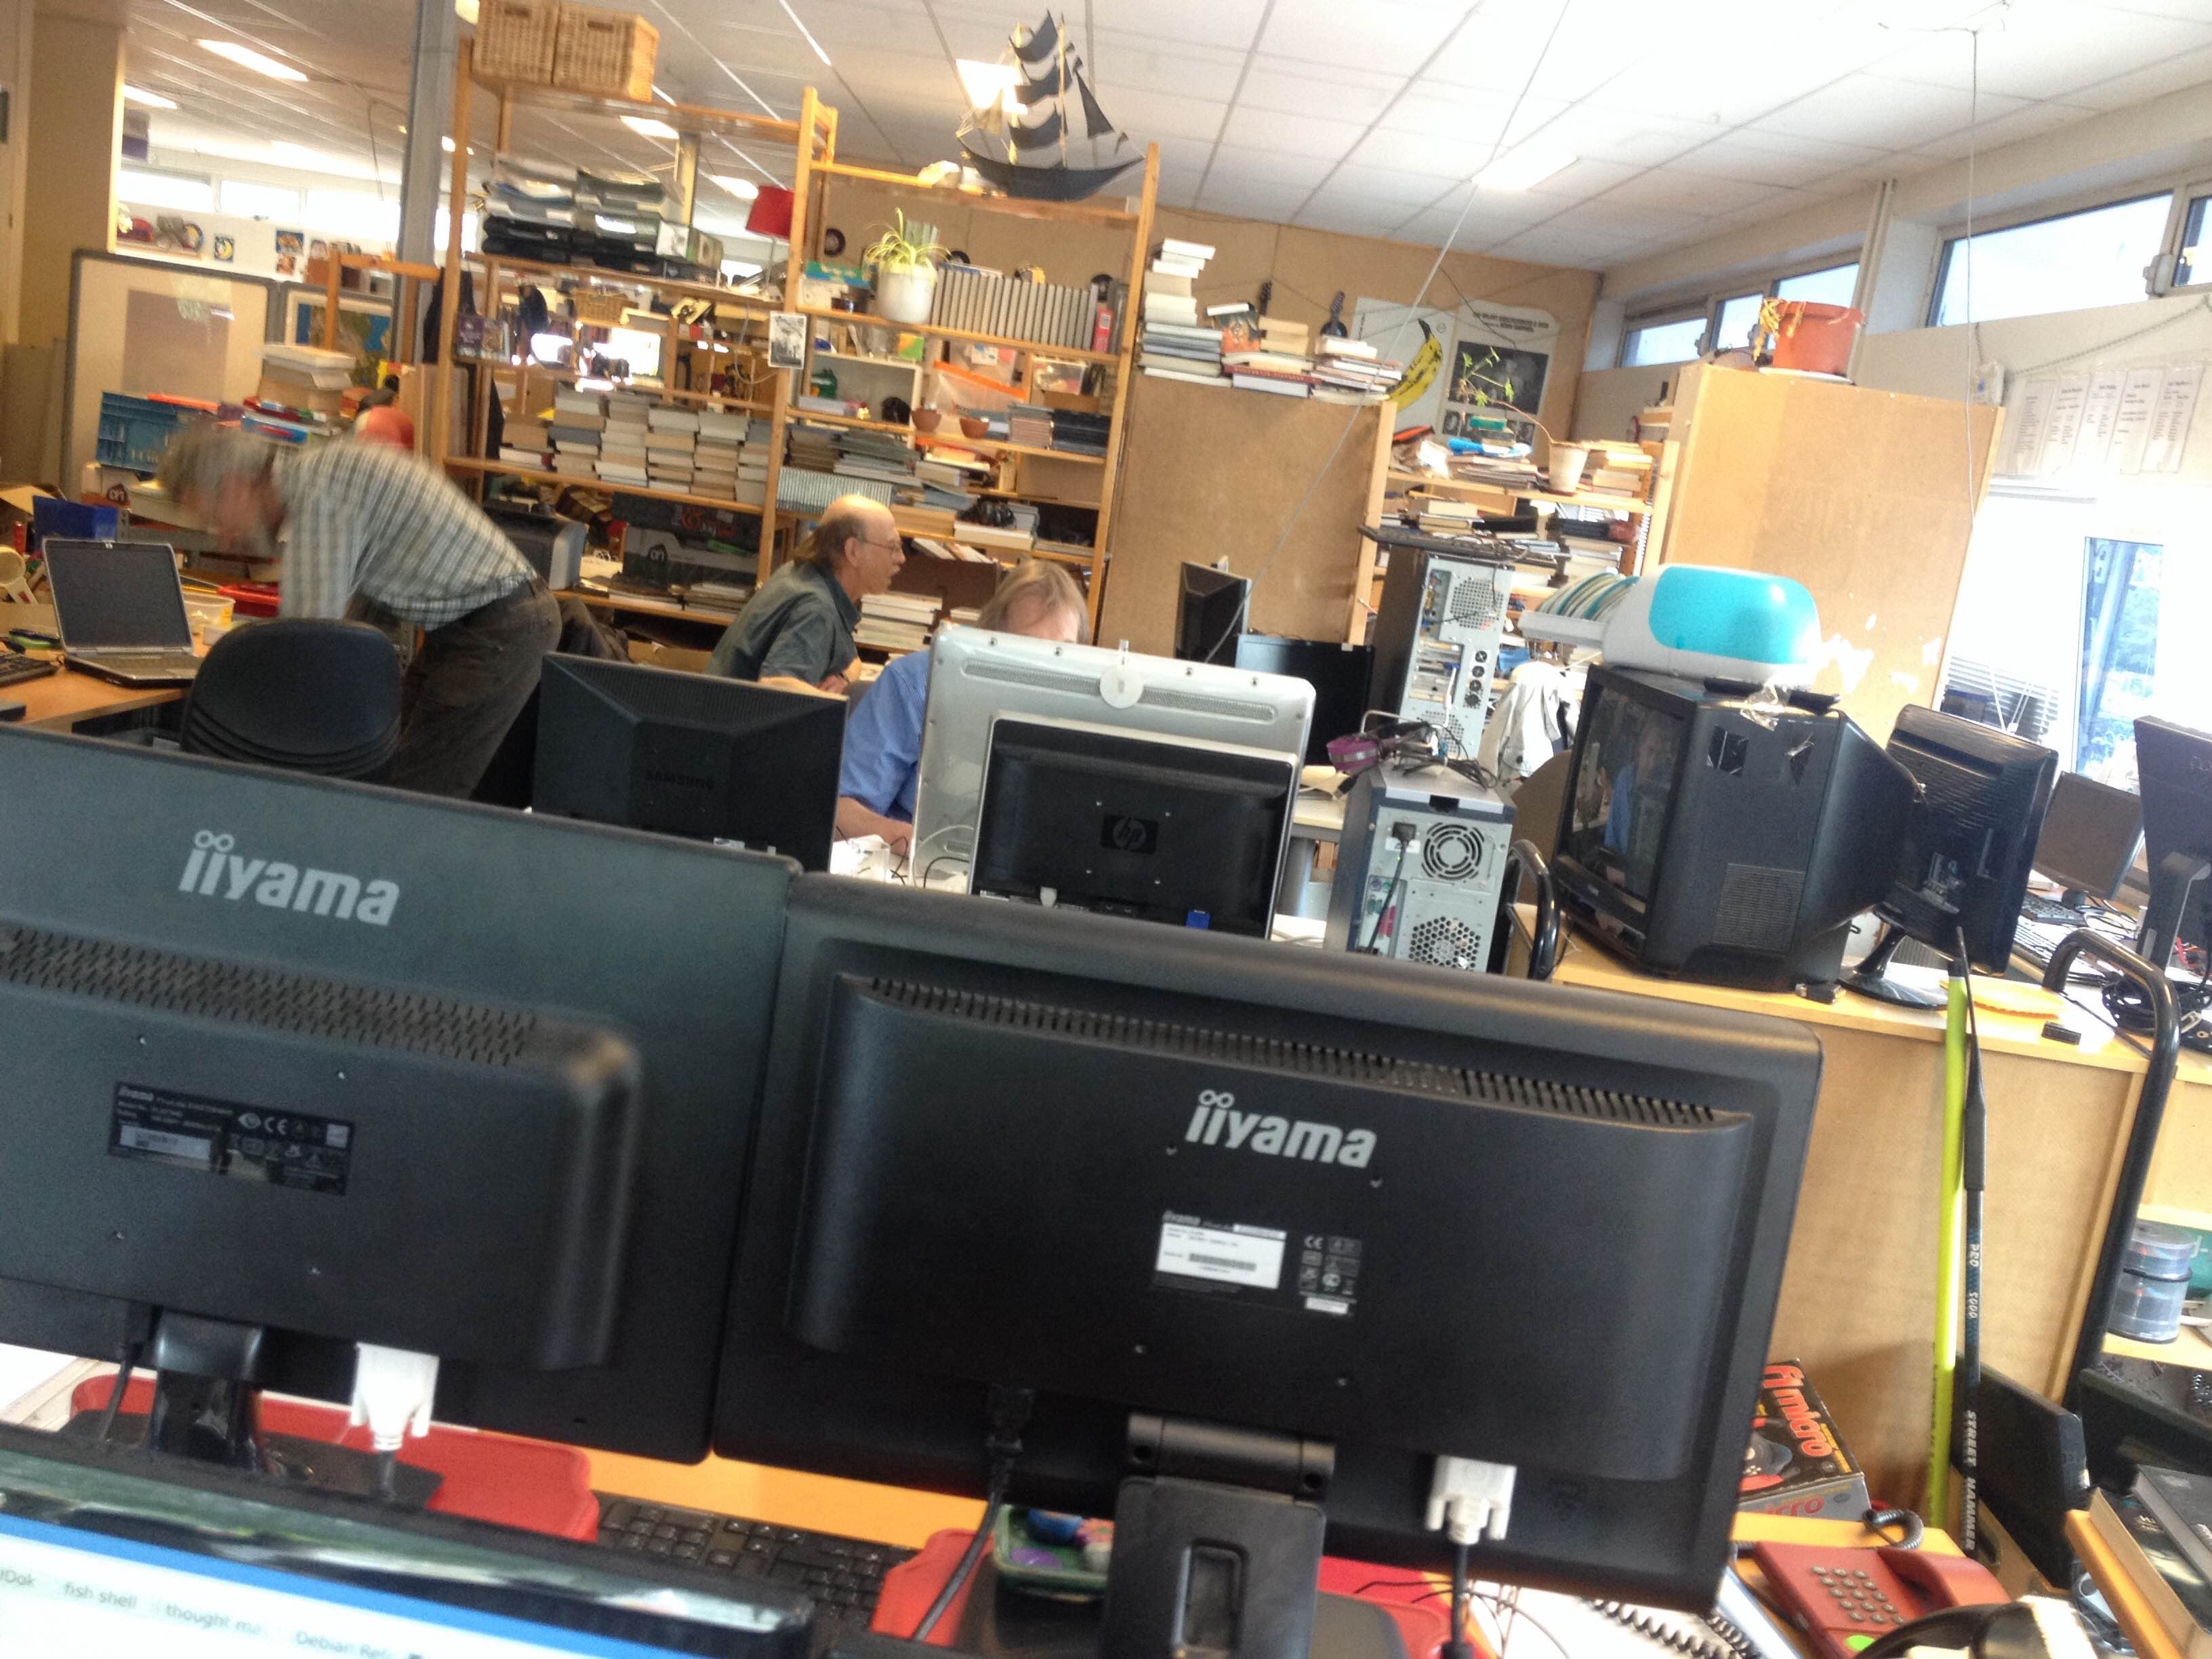
\includegraphics[width=0.80\textwidth]{IMG_4398}
\caption{Actie foto}
\end{figure}

Ik werk met \LaTeX{}.  Ik zoek dingen op op \href{https://en.wikibooks.org/wiki/LaTeX}{Latex Wikibook}.

Ik gebruik git.  De broncode van dit verslag vind je op \url{https://github.com/SilvioBos/Stageverslag}. Het artikel \href{https://guides.github.com/activities/hello-world/}{Github ''Hello world'' artikel} heb ik bestudeerd.  
Ook heb ik de volgende instructe filmpjes gekeken \href{https://www.youtube.com/watch?v=8oRjP8yj2Wo&list=PLg7s6cbtAD165JTRsXh8ofwRw0PqUnkVH}{Git Basics Training}.

\begin{figure}[H]
\centering
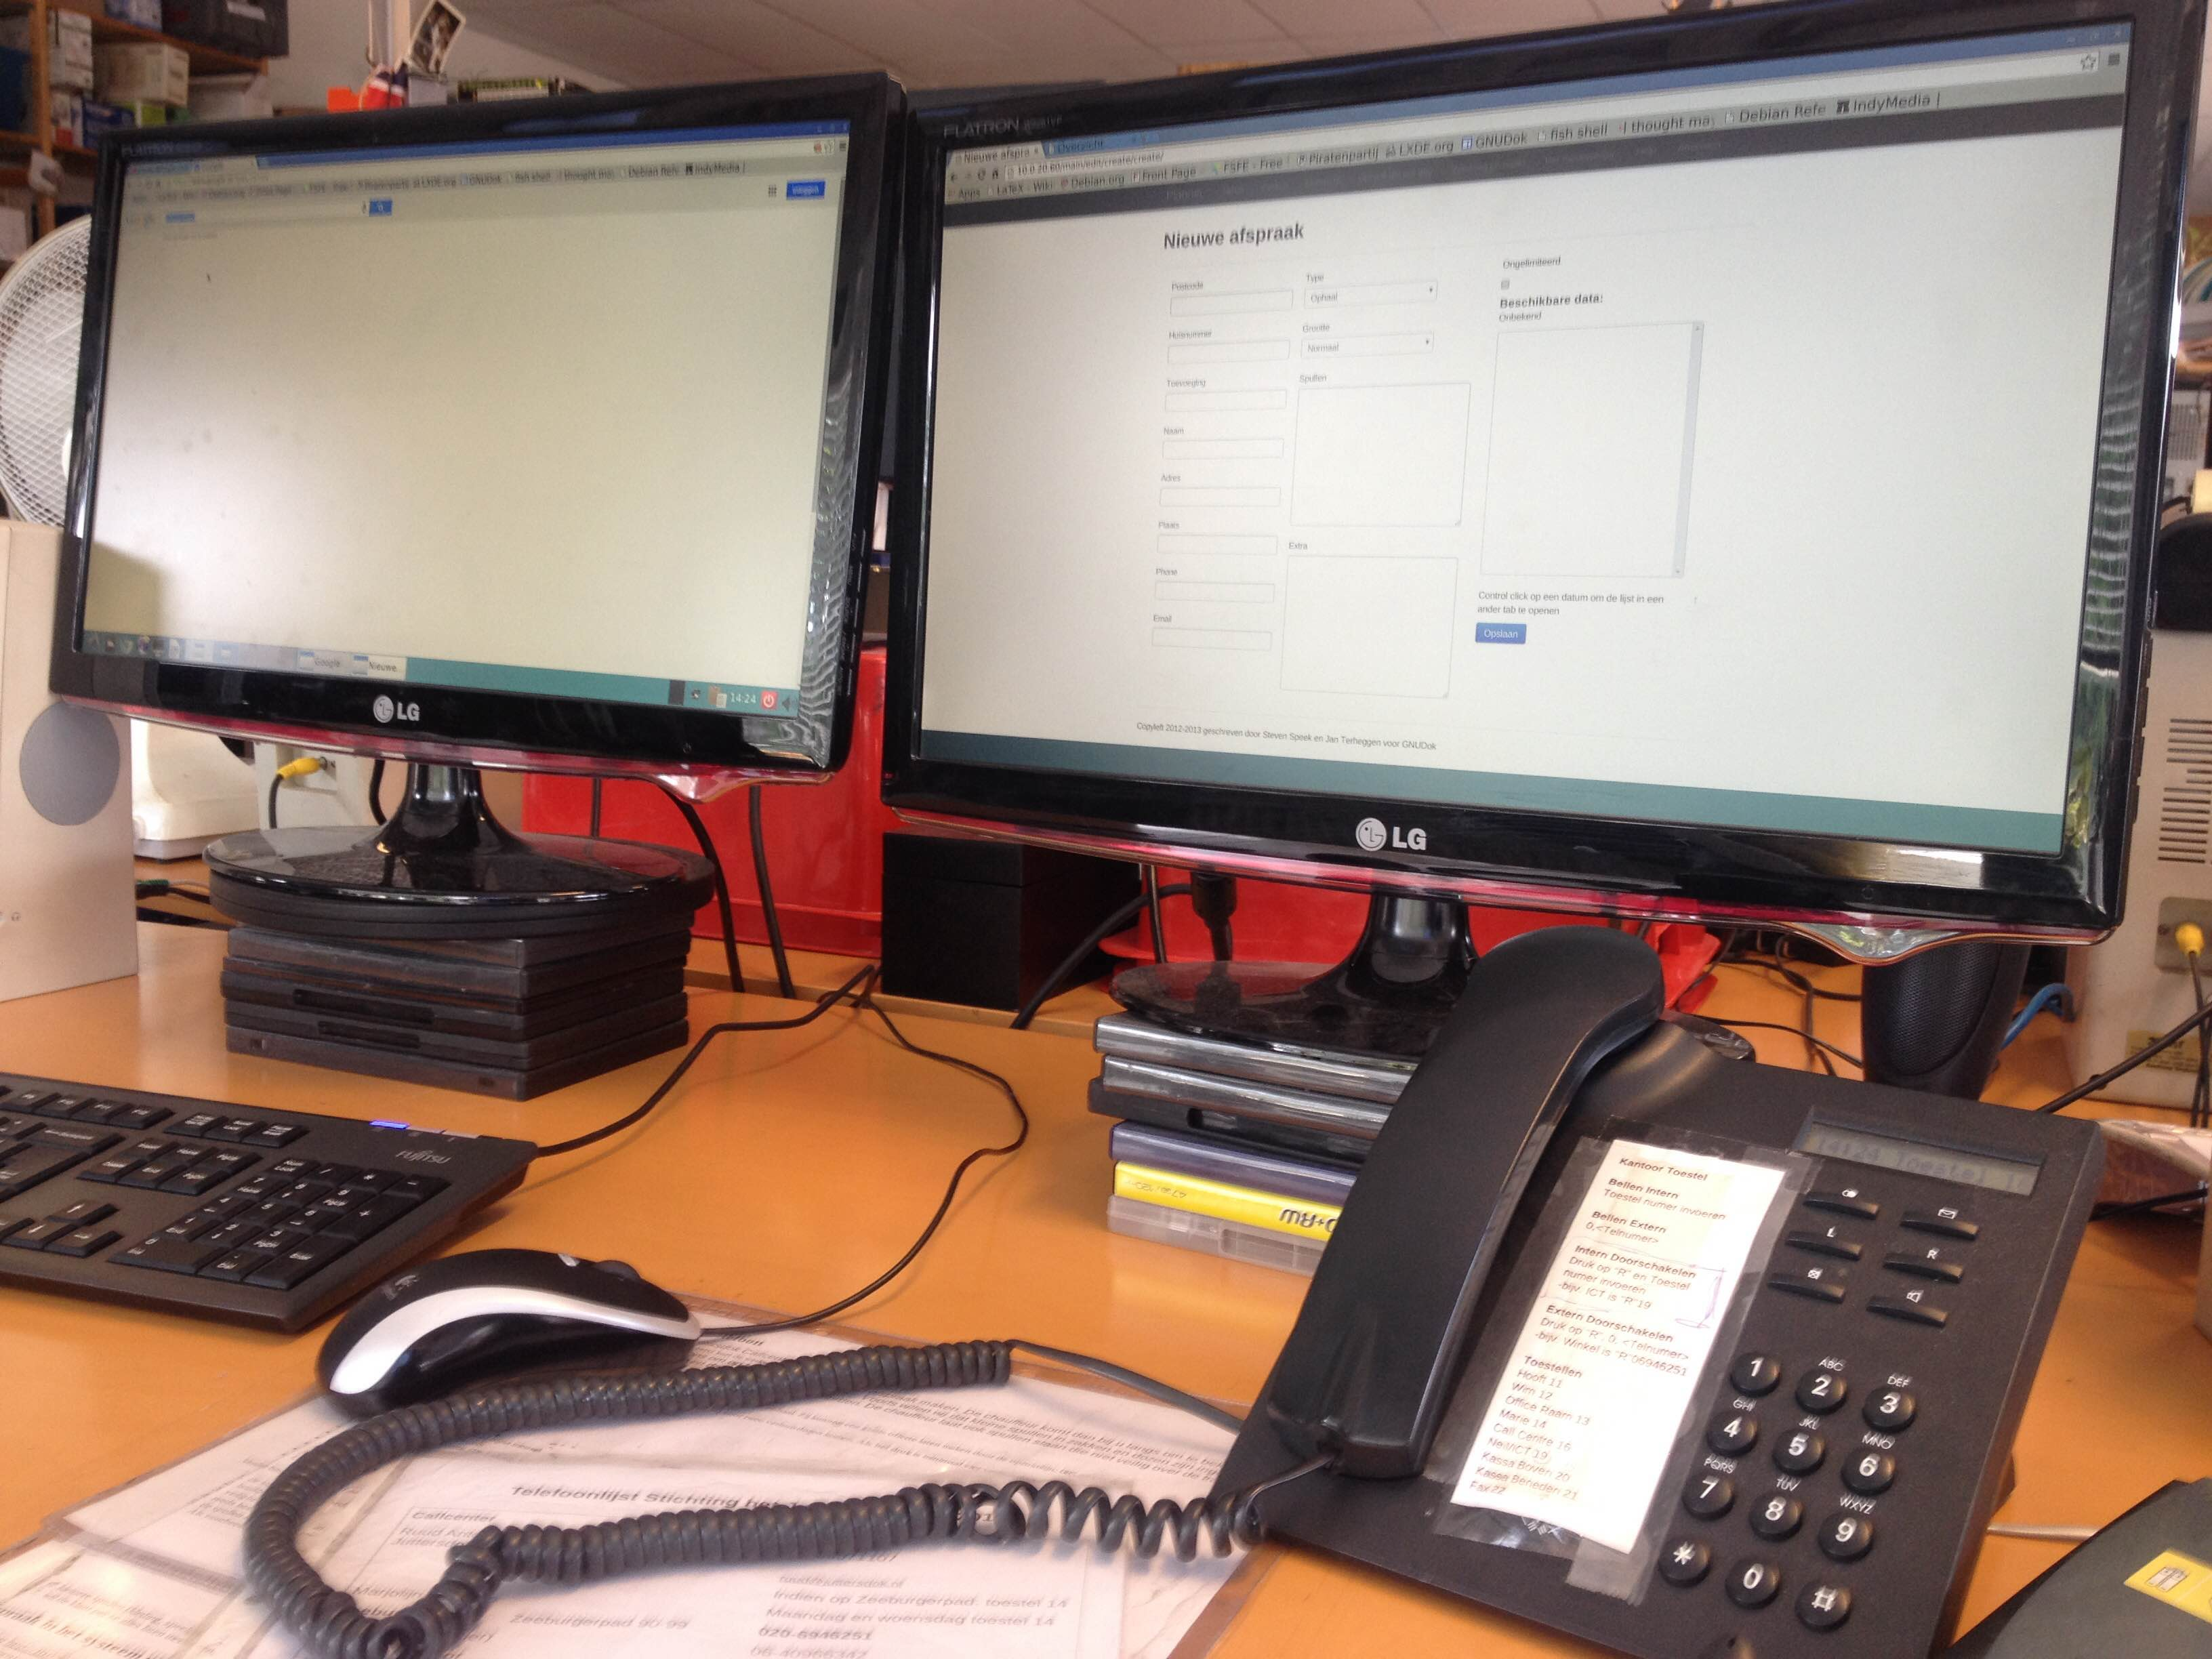
\includegraphics[width=0.80\textwidth]{IMG_4399}
\caption{Met twee grote schermen heb je wat privacy}
\end{figure}
\end{document}

